\documentclass[paper=a4, fontsize=11pt, parskip=full]{scrartcl} % A4 paper and 11pt font size

\usepackage[T1]{fontenc} % Use 8-bit encoding that has 256 glyphs
\usepackage{fourier} % Use the Adobe Utopia font for the document - comment this line to return to the LaTeX default
\usepackage[english]{babel} % English language/hyphenation
\usepackage{amsmath,amsfonts,amsthm} % Math packages

\usepackage{graphicx}

\usepackage{float}

%Preamble
\usepackage{listings}
\usepackage{color}
\definecolor{javared}{rgb}{0.6,0,0} % for strings
\definecolor{javagreen}{rgb}{0.25,0.5,0.35} % comments
\definecolor{javapurple}{rgb}{0.5,0,0.35} % keywords
\definecolor{javadocblue}{rgb}{0.25,0.35,0.75} % javadoc
 
\lstset{language=Java,
basicstyle=\ttfamily,
keywordstyle=\color{javapurple}\bfseries,
stringstyle=\color{javared},
commentstyle=\color{javagreen},
morecomment=[s][\color{javadocblue}]{/**}{*/},
numbers=left,
numberstyle=\tiny\color{black},
stepnumber=2,
numbersep=10pt,
tabsize=4,
showspaces=false,
showstringspaces=false}


\usepackage{hyperref}
\hypersetup{
    colorlinks=true,
    linkcolor=blue,
    filecolor=magenta,      
    urlcolor=cyan,
}

\usepackage{lipsum} % Used for inserting dummy 'Lorem ipsum' text into the template

\usepackage{sectsty} % Allows customizing section commands
\allsectionsfont{\centering \normalfont\scshape} % Make all sections centered, the default font and small caps

\usepackage{fancyhdr} % Custom headers and footers
\pagestyle{fancyplain} % Makes all pages in the document conform to the custom headers and footers
\fancyhead{} % No page header - if you want one, create it in the same way as the footers below
\fancyfoot[L]{} % Empty left footer
\fancyfoot[C]{} % Empty center footer
\fancyfoot[R]{\thepage} % Page numbering for right footer
\renewcommand{\headrulewidth}{0pt} % Remove header underlines
\renewcommand{\footrulewidth}{0pt} % Remove footer underlines
\setlength{\headheight}{13.6pt} % Customize the height of the header

\numberwithin{equation}{section} % Number equations within sections (i.e. 1.1, 1.2, 2.1, 2.2 instead of 1, 2, 3, 4)
\numberwithin{figure}{section} % Number figures within sections (i.e. 1.1, 1.2, 2.1, 2.2 instead of 1, 2, 3, 4)
\numberwithin{table}{section} % Number tables within sections (i.e. 1.1, 1.2, 2.1, 2.2 instead of 1, 2, 3, 4)

\setlength\parindent{0pt} % Removes all indentation from paragraphs - comment this line for an assignment with lots of text

%----------------------------------------------------------------------------------------
%	TITLE SECTION
%----------------------------------------------------------------------------------------

\newcommand{\horrule}[1]{\rule{\linewidth}{#1}} % Create horizontal rule command with 1 argument of height

\title{	
\normalfont \normalsize 
\textsc{University of Virginia, Department of Computer Science} \\ [25pt] % Your university, school and/or department name(s)
\horrule{0.5pt} \\[0.4cm] % Thin top horizontal rule
\huge Lab 01 - Introduction to Java and Eclipse \\ % The assignment title
\horrule{2pt} \\[0.5cm] % Thick bottom horizontal rule
}

\author{Dr. Mark R. Floryan} % Your name

\date{\normalsize\today} % Today's date or a custom date

\begin{document}

\maketitle % Print the title

%----------------------------------------------------------------------------------------
%	Pre-Lab
%----------------------------------------------------------------------------------------

\section{Pre-Lab}

The goal of this prelab is to setup your coding environment in eclipse, and to write a very simple program. You will do the following:

\begin{enumerate}
	\item Download and install eclipse, setup a new project.
	\item Implement a simple program that computes the power function.
	\item \textbf{FILES TO DOWNLOAD:} None
	\item \textbf{FILE TO SUBMIT:} Power.java
\end{enumerate}

%------------------------------------------------

\subsection{Download and Install Eclipse}

Eclipse is an Integrated Development Environment (IDE) for Java developers. An IDE allows programmers to code in an environment containing more advanced features than a text-editor. Eclipse also provides easy tools for managing projects, compiling code, incorporating outside libraries, etc. Your first step is to download Eclipse. You should be able to find it \href{https://www.eclipse.org/downloads/}{here}.

When you first open Eclipse, you might (depending on your version) see a welcome / tutorial screen (see figure ~\ref{fig:welcome}). If you see this screen, click on \textbf{Workbench} in the upper right corner to get to your primary work area. Your workbench, once you find it, should look like figure ~\ref{fig:workspace}.

\begin{figure}[H]
\centering
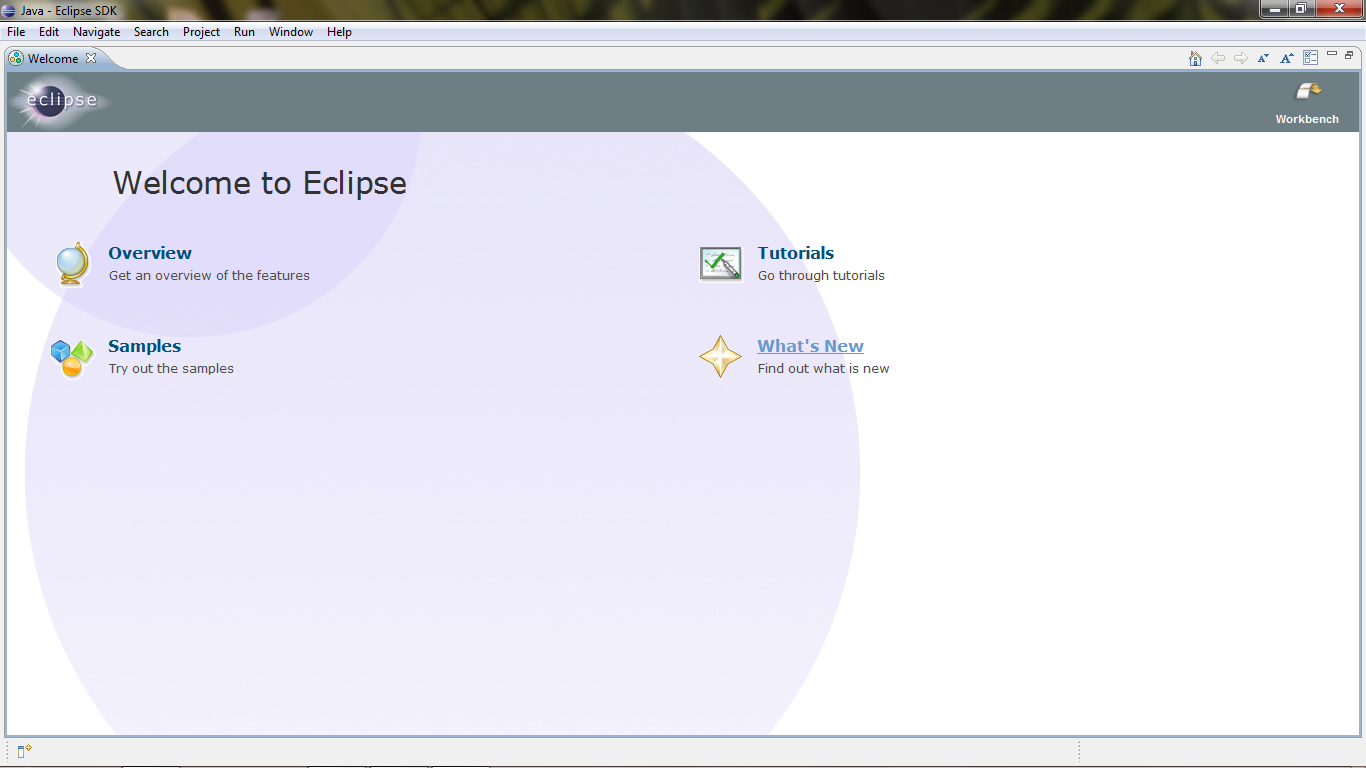
\includegraphics[width=0.7\textwidth]{images/eclipse_welcome.png}
\caption{Eclipse welcome screen}
\label{fig:welcome}
\end{figure}

\begin{figure}[H]
\centering
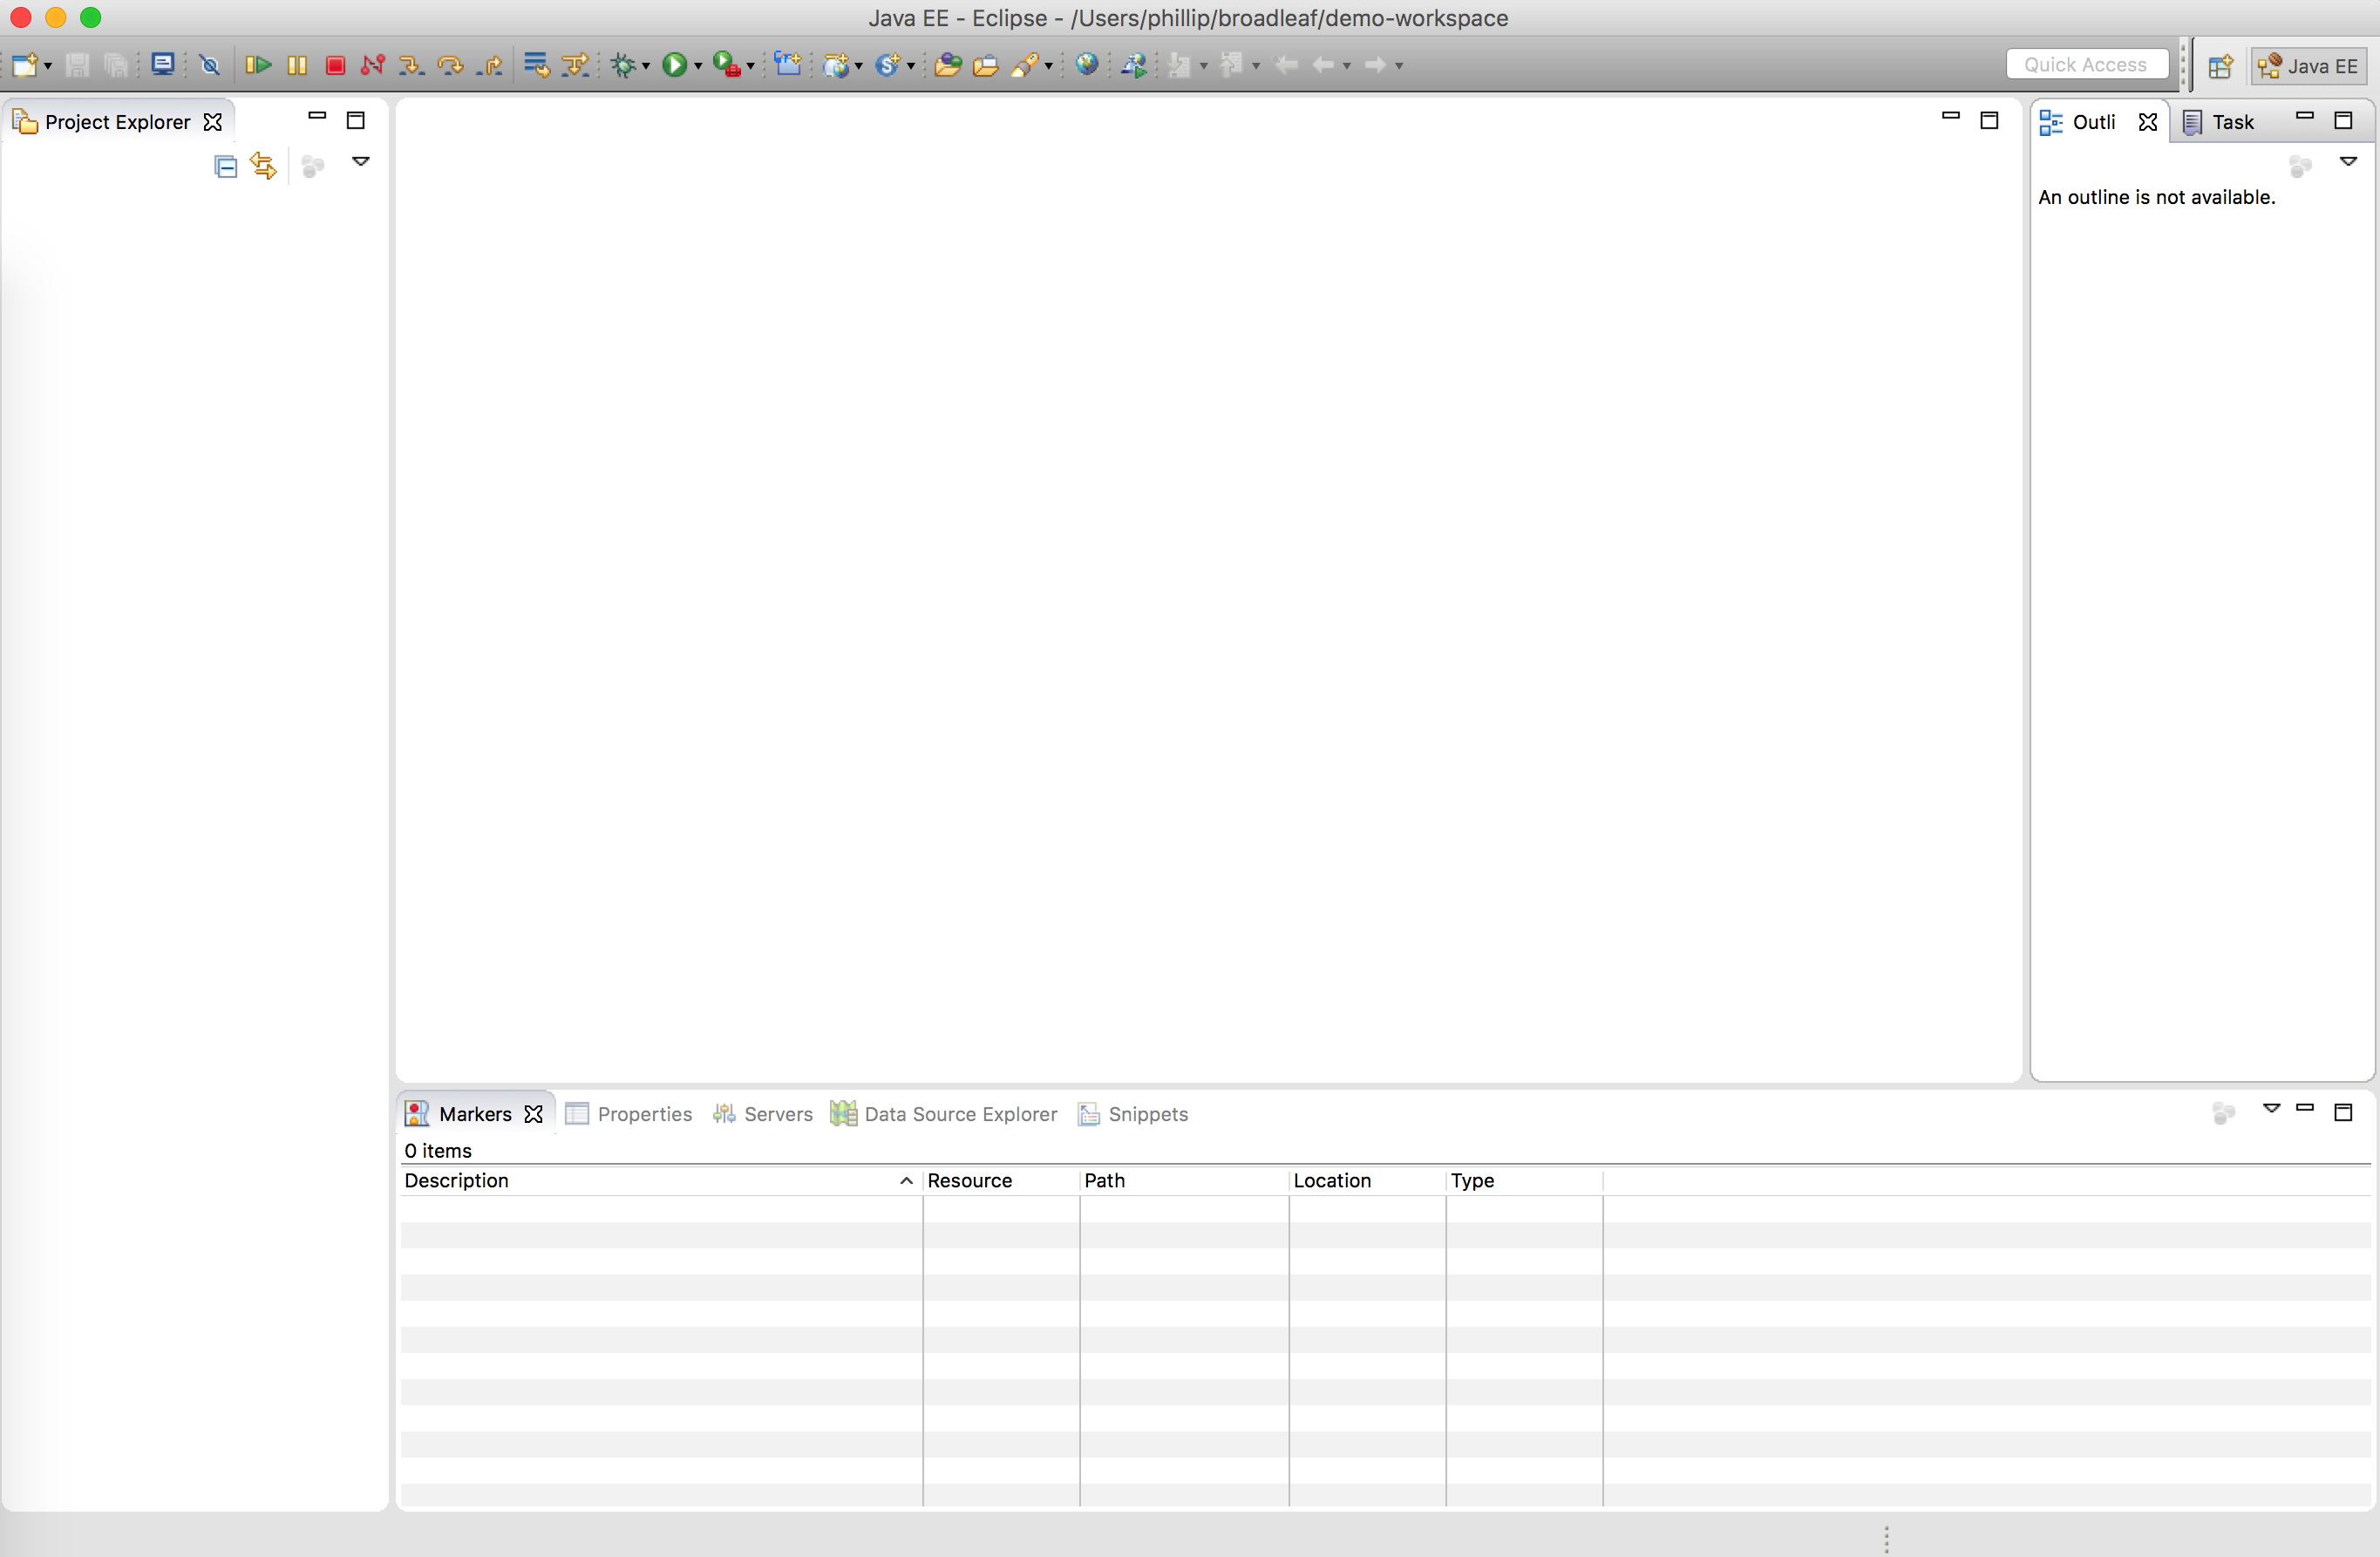
\includegraphics[width=0.7\textwidth]{images/eclipse_workspace.png}
\caption{Eclipse Workspace / Workbench}
\label{fig:workspace}
\end{figure}

To start a new project, click on \textbf{File --> New --> Java Project}. A dialog will appear. You should give your project a name, select a folder for it (optional), and click finish. You should see your project appear in the left hand dialog of the screen. If you expand the project, you should see a reference to your Java system library, as well as a folder called \textbf{src}. 

Your next task is create your first Java class. Right click on your project on the left and select \textbf{New --> Class}. A dialog will appear (see figure ~\ref{fig:newclass}), name your class \textbf{Power}, and select the check box that says \textbf{public static void main(String[] args)}. this option will create a main method automatically (though if you forget to do this, you can just type in the main method code manually).

\begin{figure}[H]
\centering
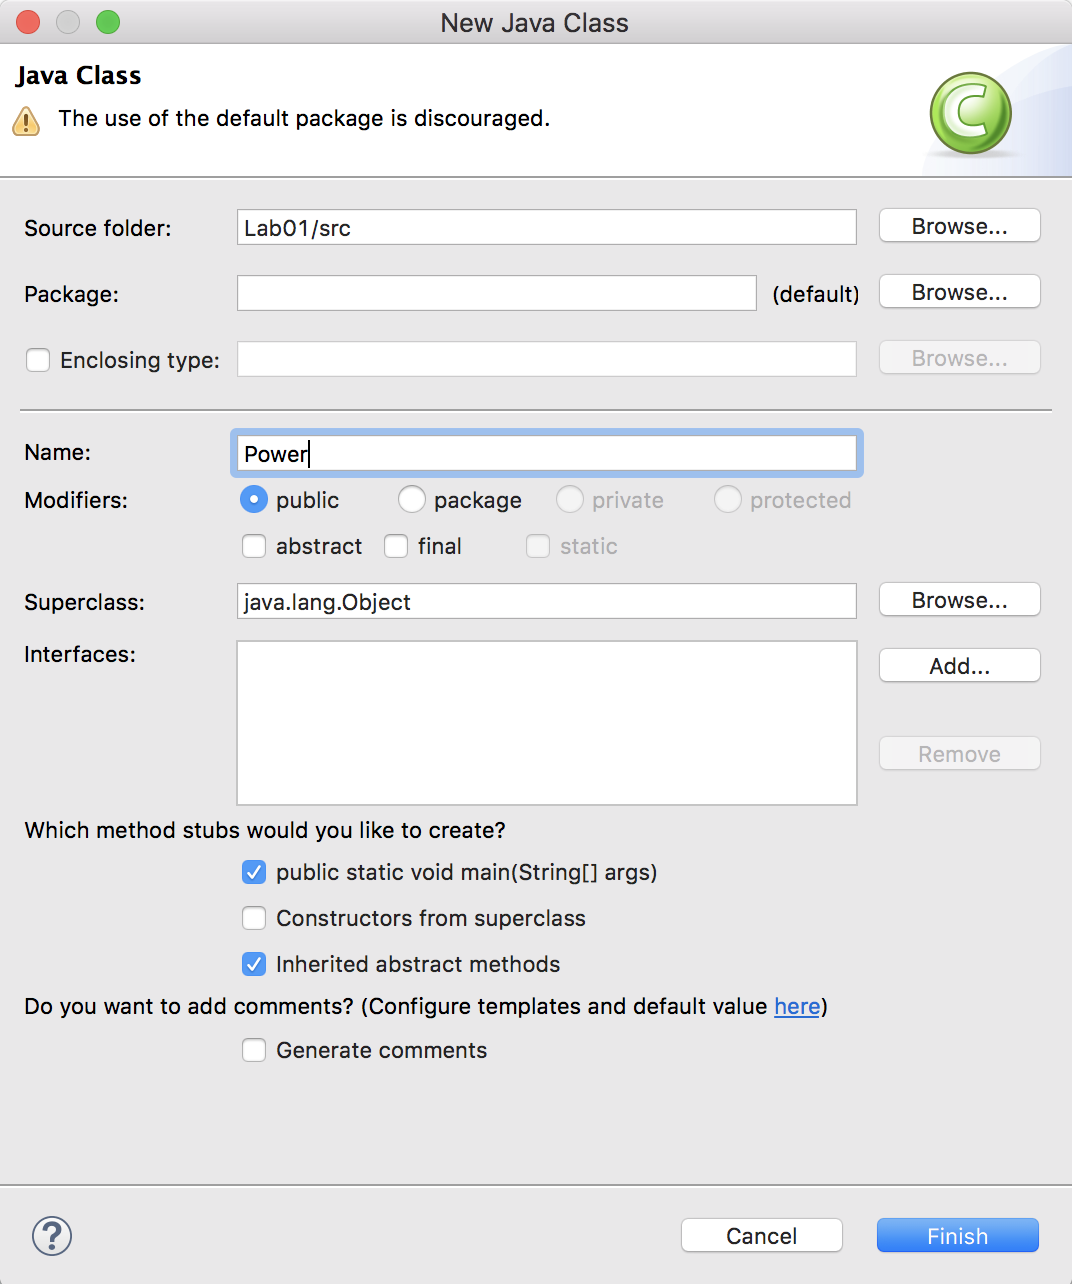
\includegraphics[width=0.4\textwidth]{images/eclipse_class_dialog.png}
\caption{New Class Dialog Screen}
\label{fig:newclass}
\end{figure}

You are ready to begin coding. For this lab, you will only need the one class, and you can write all of your code in this area. To run your program, there is a small green bug icon at the top of the screen. 


%------------------------------------------------

\subsection{Power.java}

Now that your environment is setup, you will write one very small Java method as a warm-up. The method signature is:

\begin{lstlisting}
public static long power(int base, int exp);
\end{lstlisting}

Your program should take in two numbers for the user. First, the base and second, the exponent. Then, your program should invoke the power method above and present the user (via the console) the value of base to the exponent power. You can assume that when we test your code, all inputs will fit inside of int types, and all correct answers will fit inside of long types. This method may be iterative or recursive, but \textbf{may not use any library functions such as Math.pow()}.


%----------------------------------------------------------------------------------------
%	In-Lab
%----------------------------------------------------------------------------------------
\newpage
\section{In-Lab}

The goal of this in-lab is to continue practicing writing some simple java code. You will do the following:

\begin{enumerate}
	\item Get into small groups of two
	\item The TAs will present you with various programming challenges. These will not be graded, but you are required to attend and to participate.
	\item You may think about the challenges before lab below if you'd like, but we highly recommend that you not solve them ahead of time.
	\item The TAs will give you time to solve each problem and lead you in sharing solutions with one another.
\end{enumerate}

\subsection{Programming Challenges}

The TAs will lead you in attempting to write the following methods:

\begin{enumerate}
	\item Given a list, print out the even numbered values only
	\item Given a list, print out every other element
	\item Given a list, print out only numbers that increase as you go
	\item Given two lowercase strings (a-z characters only), determine if they are anagrams of one another.
	\item Given the cost of a product $c$, and the amount a customer has paid $p$ (note $p >= c$), determine the exact coins (using quarters, dimes, nickels, and pennies) to give to produce the correct amount of change.
		\begin{itemize}
		\item If time remains, try to do each of these recursively instead of iteratively.
		\end{itemize}
	\item \textbf{Bonus Challenge}: Given the four corner points (x and y coordinates, given in clockwise order) of a polygon in two-dimensional space, and another fifth point, determine if the fifth point is inside the polygon created by the first four points.  
\end{enumerate}

%------------------------------------------------


%----------------------------------------------------------------------------------------
%	Post-Lab
%----------------------------------------------------------------------------------------
\newpage
\section{Post-Lab}

The goal of this post-lab is to continue practicing writing some simple java methods. You will do the following:

\begin{enumerate}
	\item Implement six methods shown below.
	\item Implement a small program to allow a user to choose one of those methods to invoke.
	\item \textbf{FILES TO DOWNLOAD:} None
	\item \textbf{FILE TO SUBMIT:} PostLabOne.java
\end{enumerate}

\subsection{PostLabOne.java}

For this post-lab, you will implement six functions, as well as a small program that allows a user to select which method they'd like to test. You will start by implementing the following methods:

\begin{enumerate}
\item \textbf{max}: Accepts an array of integers as a parameter, and returns the largest integer among them.
\item \textbf{min}: Accepts an array of integers as a parameter, and return the lowest integer among them.
\item \textbf{average}: Accepts an array of integers as a parameter, and returns the average of the numbers as a double.
\item \textbf{median}: Accepts an array of integers as a parameter, and returns the \href{https://en.wikipedia.org/wiki/Median}{median} of the numbers. \emph{Note that you can invoke your max and min function here to make this easier. You don't necessarily need to sort the data.} 
\item \textbf{stddev}: Accepts an array of integers as a parameter, and return the \href{https://en.wikipedia.org/wiki/Standard_deviation}{standard deviation} of the numbers. \emph{Note that you can invoke your average method here.}
\item \textbf{mode}: Accepts and array of integers as a parameter, and returns the most commonly occurring value among them. \emph{If there is more than one mode, you may return any of them.}
\end{enumerate}

Once these methods are complete, you should write a program that asks the user to input a number one through six. If the user doesn't enter a valid number, the program exits. If the user enters a valid number one through six, then they are prompted to enter seven integers. Those seven integers are then given to the corresponding method above (1 = max, 2 = min, 3 = average, 4 = median, 5 = stddev, 6 = mode) and the answer (a single value) is printed to the console. The program then exits.

You should submit one file for this lab, \textbf{PostLabOne.java}.

%------------------------------------------------

%----------------------------------------------------------------------------------------

\end{document}


%----------------------------------------------------------------------------------------
%----------------------------------------------------------------------------------------
%----------------------------------------------------------------------------------------
%----------------------------------------------------------------------------------------
%----------------------------------------------------------------------------------------
%----------------------------------------------------------------------------------------


%WORKS CITED:

%%%%%%%%%%%%%%%%%%%%%%%%%%%%%%%%%%%%%%%%%
% Short Sectioned Assignment
% LaTeX Template
% Version 1.0 (5/5/12)
%
% This template has been downloaded from:
% http://www.LaTeXTemplates.com
%
% Original author:
% Frits Wenneker (http://www.howtotex.com)
%
% License:
% CC BY-NC-SA 3.0 (http://creativecommons.org/licenses/by-nc-sa/3.0/)
%
%%%%%%%%%%%%%%%%%%%%%%%%%%%%%%%%%%%%%%%%%

%----------------------------------------------------------------------------------------
%	PACKAGES AND OTHER DOCUMENT CONFIGURATIONS
%----------------------------------------------------------------------------------------